\setModuleTitle{Understanding file system on Phoenix}
\setModuleAuthors{%
  Bowen Chen, Technology Service, University of Adelaide\\
   \mailto{bowen.chen@adelaide.edu.au}\\
}
\setModuleContributions{%
  Bowen Chen, Technology Service, University of Adelaide\\
   \mailto{bowen.chen@adelaide.edu.au} \\
}

%----------------------------------------------------------------------------------------
% MODULE TITLE PAGE
%----------------------------------------------------------------------------------------
% BEGIN: Module Title Page
%  * The chapter page will always appear on odd numbered page
\chapter{\moduleTitle}
\newpage

\section{Home directory}
%We can display a line of text in \texttt{stdout} by using the command \texttt{echo}.
%The most simple function that people learn to write in most languages is called \texttt{Hello World} and we'll do the same thing today.
On Linux, each user has a personal directory, i.e. home directory, to store his own files and data, as well as directories. 
Your home directory on Phoenix is located at /home/$\langle$userid$\rangle$. Here, /$\langle$userid$\rangle$ means aXXXXXXX, your id.\\  \\
When you login to Phoenix, your user shell is located in your home directory. The absolute pathname of your home directory, i.e. /home/$\langle$userid$\rangle$, is also stored in the environmental variable, \$HOME. Tilde symbol, $\mathtt{\sim}$, also represent your home directory. You can use following commands to change into your home directory.
\begin{steps}
\lstset{
	literate={~} {$\sim$}{1}
	}
\begin{lstlisting}
cd ~
cd $HOME
cd /home/<userid>
\end{lstlisting}
\end{steps}

\begin{information}
%There are a few subtleties about text which are worth noting.
%Inspect the \texttt{man echo} page \& note the effects of the \texttt{-e} option.
%This allows you to specify tabs, new lines \& other special characters by using the backslash to signify these characters.
%This is an important concept \& the use of a backslash to ``escape'' normal meaning of a character is very common.
%In the following, we are using the backslash to escape the normal meanings of the \texttt{t} and \texttt{n} characters, and they can take on their ``special" meaning, such as a \texttt{tab} delimiter, or a newline.
%Try the following three commands \& see what effects these special characters have.
The /home file system is backed up, and is solely intended for the files that define your user environment and irrecoverable data such as source code. The default quota of your home directory is 10 GB.
\end{information}
\begin{information}
Don't use \$HOME for launching jobs or active job data. The /home file system hardware is not designed to support the intensive file access generated by the many hundreds of jobs that run on the Phoenix compute cores, you should use the /fast file system for job input/output instead.
\end{information}

\section{Fast directory}
The /fast directory is designed to improve the data handling performance. It is supported by high performance Lustre filesystem and is intended for active job data and immediate data storage. \\
\begin{information}
%A very common process in the command line is to take the output of one process and send it to another.
%For example, we might want to cut a column from a csv file with categorical information, and then send that field to have the different categories counted by another tool.
%This is where the concept of \texttt{stdout} becomes more important. \\
The /fast directory can handle the intensive file access created by the compute jobs that run on Phoenix. It is designed to launch jobs and store personal/research data. The default quota of your fast directory is 4 TB. \\
\end{information}
Your personal fast directory is located at /fast/users/$\langle$userid$\rangle$
The absolute pathname of your fast directory is also stored in the environmental variable, \$FASTDIR
A symbolic link to that directory can be found in your home directory, i.e. $\mathtt{\sim}$/fastdir.
Thus, you can use following commands to change into your fast directory:
\begin{steps}
\lstset{
	literate={~} {$\sim$}{1}
	}
\begin{lstlisting}
cd ~/fastdir
cd $FASTDIR
cd /fast/users/<userid>
\end{lstlisting}
\end{steps}

\begin{figure}[ht]
	\centering
	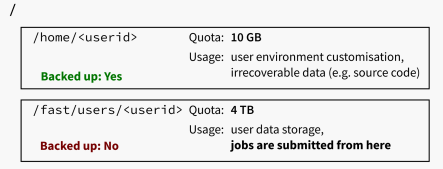
\includegraphics[width=0.9\linewidth]{images/homeFast.png} 
	\caption{Home and fast directory on Phoenix}
\end{figure}

%\begin{steps}
%By default, most command-line tools print their output to \texttt{stdout} but instead, we can send this to another tool using the pipe (\texttt{|}) symbol.
%This is exactly like putting a pipe on the output of one process, and routing it to the \textit{standard input} or \texttt{stdin} of another.
%We can use this to build up a series or chain of processes in a single line.
%A slightly ridiculous example might be to print lines 96 to 100 of the file \texttt{words} by combining \texttt{head} and \texttt{tail}
%\begin{lstlisting}
%head -n100 ~/firstname/words | tail -n5
%\end{lstlisting}
%\end{steps}

%\begin{information}
%\textbf{Note that we didn't give a file to \texttt{tail} to work with in the above command.}
%It took the \texttt{stdout} from the command \texttt{head} as it's input via \texttt{stdin}.
%This is how the pipe will work on virtually all occasions.
%\end{information}

%\begin{steps}
%As another simple example, we could take some long output from the \texttt{ls} command \& send it to the pager \texttt{less}.
%\begin{lstlisting}
%ls -lh /usr/bin | less
%\end{lstlisting}
%Page through the output until you get bored, then hit \texttt{q} to quit.
%\end{steps}

\section{Mounting filesystems}
\begin{information}
%So far, the only output we have seen has been in the terminal, i.e  \texttt{stdout}.
%Similar to the pipe command, we can redirect the output of a command \textbf{to a file} instead of \texttt{stdout}, and we do this using the greater than symbol (\textgreater), which we can almost envisage as an arrow.\\
"A file system or filesystem is used to control how data is stored and retrieved. Without a file system, information placed in a storage medium would be one large body of data with no way to tell where one piece of information stops and the next begins. By separating the data into pieces and giving each piece a name, the information is easily isolated and identified." (Wikipedia)
Mounting a filesystem simply means making the particular filesystem accessible at a certain point in the Linux directory tree.
\end{information}

\begin{steps}
You can use following commands to observe the mounting point and other information about /home and /fast on Phoenix
\end{steps}
\begin{lstlisting}
mount | egrep home
mount | egrep fast
\end{lstlisting}

%\begin{information}
%This is similar to the $>>$ trick we used earlier, but using only a single $>$ symbol will directly overwrite any existing file with the new information.
%\textbf{When using the command line, there is no }\texttt{Undo} \textbf{command.}
%Once we do something, it cannot be undone!
%\end{information}

%Once you've had a quick look at the file, exit the less pager and delete the file using the \texttt{rm} command.
%\begin{lstlisting}
%rm ampleEndings.txt
%\end{lstlisting}

\section{File and folder permissions}
Since Linux is a multi-user OS that is based on concepts of file ownership and permissions to provide security, at the file system level. Using the command, chmod, can help us to change permissions if you are the owner of the files or directories.\\
Before to use it, you need to remember several symbols and letters with the chmod. \\
\\
Identities
\begin{itemize}
\item u - the user who owns the file, i.e. owner.
\item g - the group to which the user belongs, i.e. group
\item o - others (not the owner nor the owner's group)
\item a - everyone or all (u, g, and o)
\end{itemize}

Permissions
\begin{itemize}
\item r - read access
\item w - write access
\item x - execute access
\end{itemize}

Actions
\begin{itemize}
\item + - adds the permission
\item - - removes the permission
\item = - makes it the only permission
\end{itemize}

\begin{steps}
The first thing we need to do is to create the file, foo.txt.
Use the following commands to create the file and show its default permission.
\begin{lstlisting}
touch foo.txt
ls -l foo.txt
\end{lstlisting}
When using ls -l command, you can see some thing like this: \\
-rw-r--r-- 1 a1695820 CATS\_STUDENTS 5 Sep 26 14:34 foo.txt\\
\\
Let's focus on -rw-r--r--. To explain it, parentheses will be added.\\ In -(rw-)(r--)(r--), the first pair of parentheses means the users's permission; the second means the group's permissions; the last is for all the others.\\
\\
Then using the echo command to write some words.
\begin{lstlisting}
echo "On my way to supercomputing" > foo.txt
\end{lstlisting}
Using the following command to change permissions and show current permission of it. By typing u-r, you are going to remove read permission for the user, i.e. owner, and group from the file foo.txt.
\begin{lstlisting}
chmod ug-r foo.txt
ls -l foo.txt
\end{lstlisting}
Now try to read the file with cat command
\begin{lstlisting}
cat foo.txt
\end{lstlisting}
\end{steps}

\begin{information}
When you execute commands on Phoenix, you may also meet error message like: ... Permission denied. Considering the reason caused it and how should we fix it based on what we introduced.
\end{information}

\begin{steps}
You should know what went wrong. Now let's fix the issue.
\begin{lstlisting}
ls -l foo.txt
cat foo.txt
chmod u+r foo.txt
ls -l foo.txt
cat foo.txt
\end{lstlisting}
\end{steps}

Another way to change permissions uses numeric representation.\\
Each permission setting can be represented by a numerical value:
\begin{itemize}
\item r = 4
\item w = 2
\item x = 1
\item - = 0
\end{itemize}

For example, if foo.txt has following permissions settings:\\
- (rw-) (rw-) (r--) \\
\\
Let's compute the numeric representation. The numeric representation for the user is six(4+2+0), for the group is six(4+2+0), and for others is four(4+0+0). Thus, the permissions setting is 664.\\

Bellowing is a list of common settings, numerical and meanings:
\begin{center}
	\begin{tabular}{ p{2cm}  p{3cm}  p{7cm}}
		\toprule
		\textbf{Setting} & \textbf{Numerical} & \textbf{Meaning} \\
		\midrule
		\texttt{-rw-------} & \texttt{600} & \texttt{Only owner can read and write} \\
%		\midrule
%		\texttt{.gz} & \texttt{gzip} & \texttt{gunzip} & \texttt{-d, -c, -f} \\
%								 &								& \texttt{zcat} & \\
		\midrule
		\texttt{-rw-r--r--} & \texttt{644} & \texttt{Only owner can read and write; group and others can read only} \\
		\midrule
		\texttt{-rwx------} & \texttt{700} & \texttt{Only owner can read, wirte and execute} \\
		\midrule
		\texttt{-rwxr-xr-x} & \texttt{755} & \texttt{Owner can read, wirte and execute; group and others can read and execute} \\
		\midrule
		\texttt{-rwx--x--x} & \texttt{711} & \texttt{Owner can read, wirte and execute; group and others can execute only} \\
		\midrule
		\texttt{-rw-rw-rw} & \texttt{666} & \texttt{All can read and write. (Be careful with this setting)} \\
		\midrule
		\texttt{-rwxrwxrwx} & \texttt{777} & \texttt{All can read, write and execute. (All can modify the file. Be careful.)} \\
		\bottomrule
	\end{tabular}
\end{center}

Bellowing is a list of common settings for directories:
 \begin{center}
	\begin{tabular}{ p{2cm}  p{3cm}  p{7cm}}
		\toprule
		\textbf{Setting} & \textbf{Numerical} & \textbf{Meaning} \\
		\midrule
		\texttt{-rw-------} & \texttt{600} & \texttt{Only owner can read and write in the directory} \\
		\midrule
		\texttt{-rwxr-xr-x} & \texttt{755} & \texttt{Owner can read, wirte and execute in the directory; group and others can read and execute} \\
		\bottomrule
	\end{tabular}
\end{center}


\section{Where are the applications on Phoenix?}


The applications on Phoenix are located in the /apps folder. The directory stores applications, as well as related module files. We will talk about modules on Phoenix latter.\\
%\begin{center}
%	\begin{tabular}{ p{2cm}  p{3cm}  p{3cm}   p{4cm}}
%		\toprule
%		\textbf{Suffix} & \textbf{Compress} & \textbf{Extract} & \textbf{Useful Arguments} \\
%		\midrule
%		\texttt{.zip} & \texttt{zip} & \texttt{unzip} & \texttt{-d, -c, -f} \\
%		\midrule
%		\texttt{.gz} & \texttt{gzip} & \texttt{gunzip} & \texttt{-d, -c, -f} \\
%								 &								& \texttt{zcat} & \\
%		\midrule
%		\texttt{.tar.gz} & \texttt{tar} & \texttt{tar} & \texttt{-x, -v, -f, -z} \\
%		\midrule
%		\texttt{.bz2} & \texttt{bzip2} & \texttt{bunzip2} & \\
%		\bottomrule
%	\end{tabular}
%\end{center}

%Often, files you download this way will be compressed (tar: tape archive) and archived (zipped). 
%If you see file name suffixes like .tar, .zip, .gz, and/or .bz2, among others, that is what these are.  
%To explore what these command-line options do, please check the \texttt{man} pages. \\

\begin{steps}
Let's observe the /apps directory. Firstly, list the directory's permission and what are in it.
\begin{lstlisting}
ls -ld /apps
ls -l /apps
\end{lstlisting}
You should see the two directories, modules and software. Calculating the numerical permission of the two.
Second, list what are in the directory, module
\begin{lstlisting}
ls -l /apps/modules
\end{lstlisting}
Finally, list what are in the directory, software. 
\begin{lstlisting}
ls -l /apps/modules
\end{lstlisting}
If too many things are listed, using pipe with less
\begin{lstlisting}
ls -l /apps/modules | less
\end{lstlisting}
When using less, press f key for going forward and press b key for going backward. If you want to quit, press q.
\end{steps}

%\begin{questions}
%How would we now decompress (or extract) this file?\\
%\begin{answer}
%\texttt{gunzip words.gz}\\
%\end{answer}
%
%How could we have kept our compressed file, along with the decompressed output?\\
%\begin{answer}
%\texttt{gunzip -k words.gz}\\
%\end{answer}
%
%Why would we use \texttt{zcat} instead of \texttt{gunzip -c}?\\
%\begin{answer}
%It's less typing, and it's easier to read back
%\end{answer}
%\end{questions}


%\begin{steps}
%The \texttt{GFF} file has been downloaded as a compressed file using the \texttt{gzip} program so the first thing we need to do is uncompress it.
%\begin{lstlisting}
%gunzip GCF_000011985.1_ASM1198v1_genomic.gff.gz
%\end{lstlisting}
%Don't forget to use tab auto-complete!
%\end{steps}


%\begin{steps}
%The first 7 lines of this file is what we refer to as a \textit{header}, which contains important information about how the file was generated in a standardised format.
%Many file formats have these structures at the beginning but for our purposes today we don't need to use any of this information so we can move on.
%Have a look at the beginning of the file to see what it looks like.
%\end{steps}
%\begin{lstlisting}
%head GCF_000011985.1_ASM1198v1_genomic.gff
%\end{lstlisting}

%This file begins with a few lines of header information which begin with one or two hash symbols.
%These lines contain helpful information about how the file was generated.
%The remainder of the file contains information about the genomic features themselves, in tab-separated format.
%Each line represents a genomic feature, and the tab-separated values correspond to columns in a spreadsheet.
%The first feature is annotated as a \textit{region} in the third field, whilst the second feature is annotated as a \textit{gene}.
%We'll come back to this file in the next section.
%
